\documentclass{article}
\usepackage{amsmath, amssymb, bm}
\usepackage{braket}

% Enhanced packages for better document structure
\usepackage{titlesec}
\usepackage{tocloft}
\usepackage{amsthm}
\usepackage{thmtools}
\usepackage{mdframed}
\usepackage{enumitem}
\usepackage{geometry}
\usepackage{xcolor}
\usepackage{tikz} % Added for circuit diagrams

% Set better margins
\geometry{margin=1in}

% Configure theorem-like environments
\newtheorem{theorem}{Theorem}[subsection]
\newtheorem{definition}[theorem]{Definition}
\newtheorem{example}[theorem]{Example}

% Define a nice box for important concepts
\newmdenv[
  linewidth=0.5pt,
  skipabove=1em,
  skipbelow=1em,
  backgroundcolor=gray!10,
  innerleftmargin=5pt,
  innerrightmargin=5pt,
  innertopmargin=5pt,
  innerbottommargin=5pt
]{conceptbox}

% Configure section formatting for chapters
\titleformat{\section}
  {\LARGE\bfseries}{\thesection.}{1em}{\MakeUppercase}
\titlespacing*{\section}{0pt}{3.5ex plus 1ex minus .2ex}{2.3ex plus .2ex}

% Configure subsection and subsubsection formatting
\titleformat{\subsection}
  {\Large\bfseries}{\thesubsection}{1em}{}
\titleformat{\subsubsection}
  {\large\bfseries}{\thesubsubsection}{1em}{}

% Configure spacing
\titlespacing*{\subsection}{0pt}{3.25ex plus 1ex minus .2ex}{1.5ex plus .2ex}
\titlespacing*{\subsubsection}{0pt}{3.25ex plus 1ex minus .2ex}{1.5ex plus .2ex}

% Configure list spacing
\setlist{itemsep=0.5em}

% Configure TOC depth and formatting
\setcounter{tocdepth}{3}
\renewcommand{\cftsecfont}{\Large\bfseries}
\renewcommand{\cftsecpagefont}{\bfseries}
\renewcommand{\cftsubsecindent}{2em}
\renewcommand{\cftsubsubsecindent}{4em}

\title{Advanced Electromagnetism I}
\author{PHYS 435}
\date{Fall 2025}

\begin{document}
\maketitle

\newpage
\tableofcontents
\newpage

\section{Lecture 2: Gauss's Law}
\subsubsection*{August 27, 2025}

\subsection{Gauss's Law}
\begin{conceptbox}
The electric field from a collection of charges is the vector sum of the fields from each charge.
\begin{align*}
    \vec{E} = \frac{1}{4\pi\epsilon_0}\sum_{i=1}^N \frac{q_i}{|\vec{r}_i|^2} \hat{\vec{r}}_i,\text{ } \vec{r}_i=\vec{r}-\vec{r'}_i
\end{align*}
\end{conceptbox}

\subsection{Gauss's Law in Differential Form}
\begin{conceptbox}
The divergence of the electric field is proportional to the charge density.
\begin{align*}
    \oint_C v(\vec{r}) \cdot d\vec{a} = \int_v (\mathcal{r}\cdot\vec{v}(\vec{r}))d\tau \\
    \vec{v}(\vec{r}) = \text{any differentiable vector field} \\
    \mathcal{r}\cdot\vec{v} = \text{divergence} = \frac{\partial v_x}{\partial x} + \frac{\partial v_y}{\partial y} + \frac{\partial v_z}{\partial z} \\
    \text{Apply to Gauss's Law}: \\
    \oint \vec{E} \cdot d\vec{a} = \int_v (\mathcal{r}\cdot\vec{E}(\vec{r}))d\tau = \frac{Q_{enc}}{\epsilon_0}, \text{ } Q_{enc} = \int_v \rho(\vec{r})d\tau \\
    \int_v(\mathcal{r}\cdot\vec{E})d\tau = \int_v(\rho(\vec{r})/\epsilon_0)d\tau \\
    \nabla\cdot\vec{E}(\vec{r}) = \frac{\rho(\vec{r})}{\epsilon_0} \\
    \text{Divergence Identity: }\\
    \mathcal{r}_r\cdot(\frac{\vec{r}}{r^2}) = 4\pi\delta^3(\vec{r}) \\
\end{align*}
\end{conceptbox}

\section{Lecture 3: The curl of $\vec{E}(\nabla\times\vec{E})$}
\subsubsection*{August 29, 2025}
\begin{conceptbox}
Integral:
\begin{align*}
    \oint_C \vec{E} \cdot d\vec{a} = \frac{Q_{enc}}{\epsilon_0}
\end{align*}
Differential:
\begin{align*}
    \nabla\times\vec{E}(\vec{r}) = \frac{\rho(\vec{r})}{\epsilon_0}
\end{align*}
\end{conceptbox}

\subsection{Problem 2.18 Griffiths}
Approach: Use superposition to add contributions from each sphere.

\subsection{Practice using the differential form of Gauss's Law}
\begin{example}
    For the differential form, it is important to remember we are considering a specified point in space.
\begin{align*}
    \text{Consider two identical charged plates and the electric field between them is constant.} \\
    \text{The charge density is $0$ between the plates.} \nabla\cdot\vec{E}=0, \nabla\cdot\vec{E}=\frac{\rho}{\epsilon_0} \Rightarrow \text{Charge density is 0} \\
    \nabla\cdot\vec{E}\neq0 \Rightarrow \text{charge density}
\end{align*}
\end{example}

\begin{example}
    Now consider $\nabla\times\vec{E}$ (curl)
    \begin{align*}
        \text{By Stokes's theorem: } \int_S (\nabla \times \vec{v}) \cdot d\vec{a} = \oint_C \vec{v} \cdot d\vec{l}
    \end{align*}
\end{example}
\begin{conceptbox}
The curl of any electric field due to a fixed charge distribution is zero:
\[
\nabla \times \vec{E}(\vec{r}) = 0
\]
For any closed loop,
\[
\oint \vec{E} \cdot d\vec{l} = 0
\]
\end{conceptbox}
\newpage
\section{Lecture 4: Electric Potential}
\subsubsection*{September 3, 2025}

\subsection{Electric Potential}
For static charge distributions
\begin{align*}
    \mathcal{r}\times\vec{E} = 0 \rightarrow \text{implies that 3 components of $\vec{E}$ are related to each other.}
\end{align*}
Stokes's Theorem states that:
\begin{center}
\begin{align*}
    &\int_S (\mathcal{r} \times \vec{E}) \cdot d\vec{a} = \oint_P \vec{E} \cdot d\vec{l} \\[1.5ex]
    &\oint_P \vec{E} \cdot d\vec{l} = 0 \\[1.5ex]
    &\oint_P \vec{E} \cdot d\vec{l} \text{ is independent of path} \\[1.5ex]
    &\int_a^b \vec{E} \cdot d\vec{l} + \int_b^a \vec{E} \cdot d\vec{l} = 0 \\[1.5ex]
    &\text{Only the endpoints $a$ and $b$ matter} \\[1.5ex]
    &\text{We can define a scalar function $V(\vec{r})$ such that:} \\[0.5ex]
    &\int_a^b \vec{E} \cdot d\vec{l} = V(\vec{a}) - V(\vec{b}) \\
    &V(\vec{r}) = - \int_a^r \vec{E} \cdot d\vec{l} \\
    &V(b)-V(a)=-\int_0^b \vec{E} \cdot d\vec{l}+\int_0^a \vec{E} \cdot d\vec{l}=-\int_a^b \vec{E} \cdot d\vec{l} \\
    &\text{Fundamental thereom of gradients: } V(b)-V(a)=\int_a^b\nabla V\cdot d\vec{l} \\
    &\rightarrow \vec{E}=-\nabla V(\vec{r})
\end{align*}
\end{center}

\subsection{Potential}
\begin{center}
\begin{align*}
    &\text{1. $V$ is the (electric) potential.} \\
    &E = \frac{N}{C}, \quad V = \frac{N \cdot m}{C} = \frac{J}{C} = \text{Volt} \\
    &\text{2. The potential at one point has no physical significance.} \\
    &\text{Potential differences matter. We always define some reference point $O$.} \\
    &\text{Typically choose $O$ such that $V(O)=0$. We can always change the} \\
    &\text{reference point if we wish $V(\vec{r})\rightarrow V(\vec{r})+C$.} \\
    &\vec{E}\rightarrow\vec{E} \\
    &\text{3. Superposition also works with the potential} \\
    &\vec{E}=\vec{E}_1+\vec{E}_2+\cdots+\vec{E}_N \\
    &\vec{E}=-\nabla V \text{ or } V(\vec{r})=-\int_0^r \vec{E} \cdot d\vec{l} \\
    &V_{total}=-\int_0^r \vec{E}_1 \cdot d\vec{l} + -\int_0^r \vec{E}_2 \cdot d\vec{l} + \cdots + -\int_0^r \vec{E}_N \cdot d\vec{l} \\
    &= v_1(\vec{r}) + v_2(\vec{r}) + \cdots + v_N(\vec{r}) \\
\end{align*}
\end{center}
\example[Potential due to a point charge]

\begin{center}
\begin{minipage}{0.45\textwidth}
    \begin{center}
    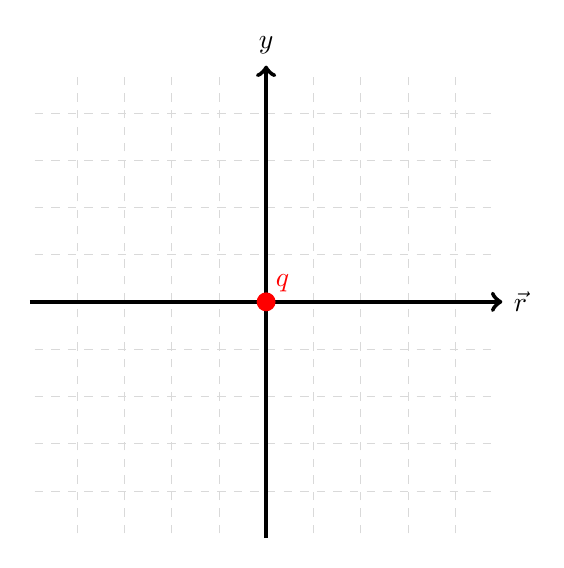
\begin{tikzpicture}[scale=0.6]
        \draw[help lines, color=gray!30, dashed] (-4.9,-4.9) grid (4.9,4.9);
        \draw[->,ultra thick] (-5,0)--(5,0) node[right]{$\vec{r}$};
        \draw[->,ultra thick] (0,-5)--(0,5) node[above]{$y$};
        \fill[red] (0,0) circle (0.2) node[above right]{$q$};
    \end{tikzpicture}
    \end{center}
\end{minipage}
\hfill
\begin{minipage}{0.45\textwidth}
    \begin{align*}
        &\vec{E}=\frac{q}{4\pi\epsilon_0}\frac{1}{r^2}\vec{r} \\
        &V(\vec{r})=-\int_0^{\vec{r}} \vec{E} \cdot d\vec{l} \\
        &=-\int_{\infty}^r \frac{q}{4\pi\epsilon_0}\frac{1}{r'^2} dr' \\
        &=\frac{q}{4\pi\epsilon_0}\frac{1}{r}
    \end{align*}
\end{minipage}
\end{center}

\subsection{Poisson's Equation}
\begin{align*}
    \vec{E}=-\nabla V, \text{Gauss's law} \nabla\cdot\vec{E}(\vec{r})=\frac{\rho(\vec{r})}{\epsilon_0} \rightarrow \nabla^2 V = \frac{\rho(\vec{r})}{\epsilon_0} + \text{Boundary conditions}
\end{align*}

\newpage
\section{Lecture 5: Electrostatic Boundary Conditions}
\subsubsection*{September 5, 2025 \\}

Recall: $\vec{E}(\vec{r}) = -\nabla V(\vec{r})$, and also $\nabla^2 V(\vec{r}) = \frac{\rho(\vec{r})}{\epsilon_0}$. \\

Invert: $\nabla^2 V(\vec{r}) = -\frac{\rho(\vec{r})}{\epsilon_0} \rightarrow V(\vec{r}) = f(p)$. \\

For a point charge, $V(\vec{r}) = \frac{q}{4\pi\epsilon_0 \mathcal{r}}$, where $\vec{\mathcal{r}} = \vec{r} - \vec{r}'$. \\

If we add another charge, $V(\vec{r}) = \frac{q}{4\pi\epsilon_0 \mathcal{r}} + \frac{q'}{4\pi\epsilon_0 \mathcal{r}'}$ (just superpose). \\

For $N$ charges: $V(\vec{r}) = \sum_{i=1}^N \frac{q_i}{4\pi\epsilon_0 \mathcal{r}_i}$. \\

For a continuous distribution: $V(\vec{r}) = \int \frac{dq}{4\pi\epsilon_0 \mathcal{r}} = \int \frac{\rho(\vec{r}')}{4\pi\epsilon_0 \mathcal{r}} d\tau'$. \\

For a line charge: $V(\vec{r}) = \int \frac{\lambda(\vec{r}')}{4\pi\epsilon_0 \mathcal{r}} dl'$. \\

For a surface charge: $V(\vec{r}) = \int \frac{\sigma(\vec{r}')}{4\pi\epsilon_0 \mathcal{r}} da'$. \\

For a volume charge: $V(\vec{r}) = \int \frac{\rho(\vec{r}')}{4\pi\epsilon_0 \mathcal{r}} d\tau'$.

\newpage
\subsection{Line Charge}
\example[Find e-field from line charge]

\begin{center}
\begin{minipage}{0.48\textwidth}
    \centering
    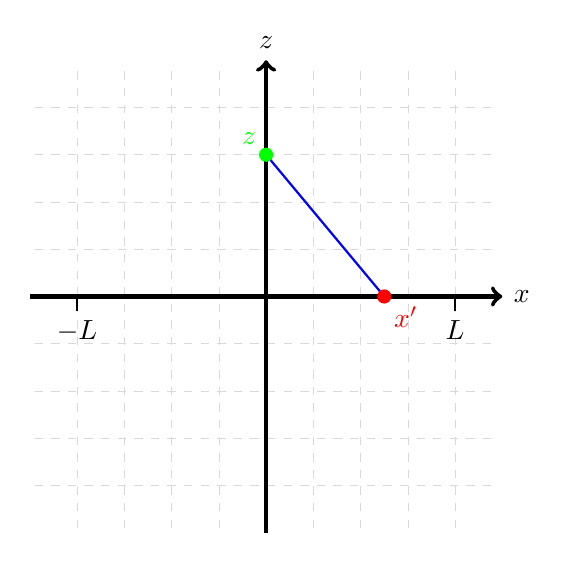
\begin{tikzpicture}[scale=0.6]
        \draw[help lines, color=gray!30, dashed] (-4.9,-4.9) grid (4.9,4.9);
        \draw[->,ultra thick] (-5,0)--(5,0) node[right]{$x$};
        \draw[->,ultra thick] (0,-5)--(0,5) node[above]{$z$};
        \draw[thick] (-4,0) -- (-4,-0.3) node[below]{$-L$};
        \draw[thick] (4,0) -- (4,-0.3) node[below]{$L$};
        \coordinate (xprime) at (2.5,0);
        \coordinate (zpoint) at (0,3);
        \draw[thick, blue] (xprime) -- (zpoint);
        \fill[red] (xprime) circle (0.15) node[below right]{$x'$};
        \fill[green] (zpoint) circle (0.15) node[above left]{$z$};
    \end{tikzpicture}
\end{minipage}%
\hfill
\begin{minipage}{0.48\textwidth}
    \vspace{0.5em}
    \begin{align*}
        &\int dV = \int \frac{dq}{4\pi\epsilon_0\mathcal{r}} = \int \frac{\lambda dx'}{4\pi\epsilon_0\sqrt{x'^2+z^2}} \\
        &V = \frac{\lambda}{4\pi\epsilon_0} \int_{-L}^L \frac{dx'}{\sqrt{x'^2+z^2}} = \frac{\lambda}{4\pi\epsilon_0} \left[\ln(x'+\sqrt{x'^2+z^2})\right]_{-L}^L \\
        &V(z) = \frac{\lambda}{4\pi\epsilon_0} \ln\left(\frac{L+\sqrt{L^2+z^2}}{-L+\sqrt{L^2+z^2}}\right) \\
        &\vec{E}=-\nabla V = -(\frac{\partial V}{\partial x}\hat{x}+\frac{\partial V}{\partial y}\hat{y}+\frac{\partial V}{\partial z}\hat{z}) = -\frac{\partial V}{\partial z}\hat{z} = \frac{2L\lambda}{4\pi\epsilon_0} \frac{1}{z\sqrt{L^2+z^2}} \hat{z} \\
    \end{align*}
\end{minipage}
\end{center}

\newpage
\subsection{Spherical Shell}

\begin{example}[Spherical Shell]
\begin{center}
\begin{minipage}{0.48\textwidth}
    \centering
    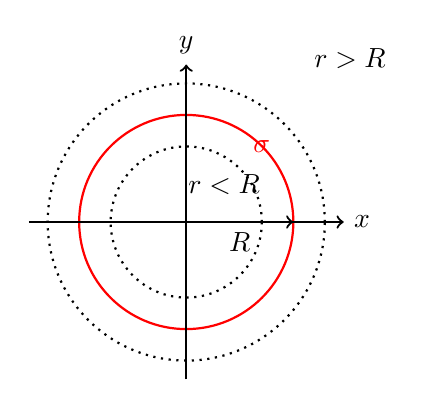
\begin{tikzpicture}[scale=0.8]
        % Draw dotted circles smaller and larger than the shell
        \draw[dotted, thick] (0,0) circle (1.2);
        \draw[dotted, thick] (0,0) circle (2.2);
        
        % Draw the main spherical shell with radius R
        \draw[thick, red] (0,0) circle (1.7);
        
        % Add surface charge density label
        \node[red] at (1.2, 1.2) {$\sigma$};
        
        % Add radius label
        \draw[thick, ->] (0,0) -- (1.7,0) node[midway, below]{$R$};
        
        % Add labels for the dotted circles
        \node at (0.6, 0.6) {$r < R$};
        \node at (2.6, 2.6) {$r > R$};
        
        % Add coordinate axes
        \draw[->, thick] (-2.5,0) -- (2.5,0) node[right]{$x$};
        \draw[->, thick] (0,-2.5) -- (0,2.5) node[above]{$y$};
    \end{tikzpicture}
\end{minipage}%
\hfill
\begin{minipage}{0.48\textwidth}
    \vspace{0.5em}
    \begin{align*}
        &\text{Spherical shell with radius } R \text{ and surface charge density } \sigma \\
        &\text{For } r < R: \quad Q_{enc}=0, \quad \vec{E} = 0 \\
        &\text{For } r > R: \quad \oint\vec{E}\cdot d\vec{a}=\frac{Q_{enc}}{\epsilon_0}, \quad \vec{E} = \frac{\sigma}{\epsilon_0}\frac{R^2}{r^2} \hat{r} \quad \text{where } Q_{enc} = 4\pi R^2 \sigma\\
        &\text{At } r = R: \quad E_{\text{out}} - E_{\text{in}} = \frac{\sigma}{\epsilon_0} \\
        &\text{Since } E_{\text{in}} = 0: \quad E_{\text{out}} = \frac{\sigma}{\epsilon_0}
    \end{align*}
\end{minipage}
\end{center}

\vspace{1em}

\begin{center}
\begin{tikzpicture}[scale=1.1]
    % Axes
    \draw[->, thick] (0,0) -- (5.2,0) node[right] {$r$};
    \draw[->, thick] (0,0) -- (0,3.2) node[above] {$E$};

    % E field: E=0 for r<R, jump at R, then decays as 1/r^2
    \draw[thick, blue] (0,0) -- (2,0); % E=0 for r<R

    % Vertical jump at r=R
    \draw[dashed] (2,0) -- (2,2.5);
    \filldraw[black] (2,2.5) circle (1.2pt);

    % Label R on x-axis
    \draw (2,-0.15) -- (2,0.15);
    \node[below] at (2,0) {$R$};

    % Label delta E at (R, E)
    \node[right] at (2.05,2.5) {$\Delta E = \frac{\sigma}{\epsilon_0}$};

    % E for r>R: decays as 1/r^2, but for sketch, just a curve
    \draw[thick, blue, domain=2:5, samples=100] plot (\x,{2.5*4/(\x*\x)});

    % Dotted line at E = sigma/epsilon_0
    \draw[dotted] (0,2.5) -- (2,2.5);

    % Label E axis at delta E
    \node[left] at (0,2.5) {$\frac{\sigma}{\epsilon_0}$};
\end{tikzpicture}
\end{center}
\end{example}

\newpage
\subsection{Sheet of Charge}
\begin{example}[Imagine sheet of charge]
\begin{center}
\begin{minipage}{0.48\textwidth}
    \centering
    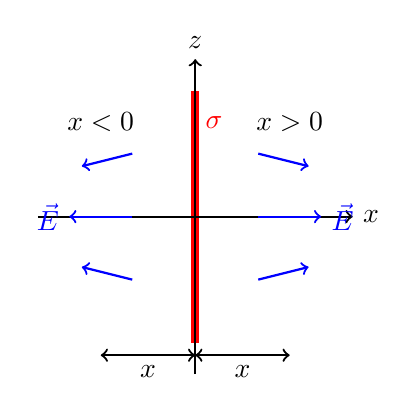
\begin{tikzpicture}[scale=0.8]
        % Draw the sheet of charge (vertical line)
        \draw[thick, red, line width=3pt] (0,-2) -- (0,2);
        
        % Add surface charge density label
        \node[red] at (0.3, 1.5) {$\sigma$};
        
        % Draw coordinate axes
        \draw[->, thick] (-2.5,0) -- (2.5,0) node[right]{$x$};
        \draw[->, thick] (0,-2.5) -- (0,2.5) node[above]{$z$};
        
        % Draw electric field lines
        \draw[->, thick, blue] (1,0) -- (2,0) node[right]{$\vec{E}$};
        \draw[->, thick, blue] (-1,0) -- (-2,0) node[left]{$\vec{E}$};
        \draw[->, thick, blue] (1,1) -- (1.8,0.8);
        \draw[->, thick, blue] (-1,1) -- (-1.8,0.8);
        \draw[->, thick, blue] (1,-1) -- (1.8,-0.8);
        \draw[->, thick, blue] (-1,-1) -- (-1.8,-0.8);
        
        % Add labels for regions
        \node at (1.5, 1.5) {$x > 0$};
        \node at (-1.5, 1.5) {$x < 0$};
        
        % Add distance labels
        \draw[<->, thick] (0,-2.2) -- (1.5,-2.2) node[midway, below]{$x$};
        \draw[<->, thick] (0,-2.2) -- (-1.5,-2.2) node[midway, below]{$x$};
    \end{tikzpicture}
\end{minipage}%
\hfill
\begin{minipage}{0.48\textwidth}
    \vspace{0.5em}
    \begin{align*}
        &\text{Infinite sheet of charge with surface density } \sigma \\
        &\text{Using Gauss's law with cylindrical Gaussian surface:} \\
        &\oint \vec{E} \cdot d\vec{a} = \frac{Q_{enc}}{\epsilon_0} \\
        &E \cdot 2A = \frac{\sigma A}{\epsilon_0} \\
        &E = \frac{\sigma}{2\epsilon_0} \\
        &\text{For } x > 0: \quad \vec{E} = \frac{\sigma}{2\epsilon_0} \hat{x} \\
        &\text{For } x < 0: \quad \vec{E} = -\frac{\sigma}{2\epsilon_0} \hat{x} \\
        &\text{Magnitude: } |E| = \frac{\sigma}{2\epsilon_0} \text{ (constant)}
    \end{align*}
\end{minipage}
\end{center}
\end{example}

\subsubsection{Loop}
$\oint \vec{E} \cdot d\vec{l} = 0$ \\
$=E^{''}_{above}l-E^{''}_{below}l=0$ $\rightarrow$ $E^{''}_{above}=E^{''}_{below}$
\subsubsection{General Statement}
$\vec{E}_{above}-\vec{E}_{below}=\frac{\sigma}{\epsilon_0}\hat{n}$, $\hat{n}$ is a unit vector defining the surface normal..

\newpage
\section{Lecture 6: Electrostatic Energy}
\subsubsection*{September 8, 2025}

\subsection{Recap: Boundary Conditions}
From the previous lecture, we found the boundary conditions at a sheet of charge:
\begin{align}
    \vec{E}_{\text{above}} - \vec{E}_{\text{below}} &= \frac{\sigma}{\epsilon_0}\hat{n} \\
    \nabla V_{\text{above}} - \nabla V_{\text{below}} &= -\frac{\sigma}{\epsilon_0}\hat{n} \\
    \frac{\partial V}{\partial n}\bigg|_{\text{above}} - \frac{\partial V}{\partial n}\bigg|_{\text{below}} &= -\frac{\sigma}{\epsilon_0}
\end{align}
where $\hat{n}$ is an outward pointing normal and $\frac{\partial V}{\partial n} = \nabla V \cdot \hat{n}$.

\subsection{Work and Potential Energy}
How much energy does it take to move a charge from point $a$ to point $b$?

For a charge $q$ in an electric field:
\begin{align}
    \vec{F}(\vec{r}) &= q\vec{E}(\vec{r}) \\
    \vec{F}_{\text{ext}} &= -q\vec{E}(\vec{r}) \quad \text{(external force needed)}
\end{align}

The work done by the external force:
\begin{align}
    W &= \int_a^b \vec{F}_{\text{ext}} \cdot d\vec{l} = -q\int_a^b \vec{E} \cdot d\vec{l} \\
    &= q[V(b) - V(a)] \quad \text{(conservative force)}
\end{align}

\textbf{Key insight:} The potential $V(\vec{r})$ has units of $\frac{\text{energy}}{\text{charge}}$. If we set the reference point at infinity where $V(\infty) = 0$, then:
\begin{equation}
    W(\vec{r}) = qV(\vec{r})
\end{equation}

\subsection{Energy in Discrete Charge Arrangements}
Imagine we are in a vacuum with no initial fields.

\textbf{Step 1:} Bring in charge $q_1$ at location $\vec{r}_1$
\begin{equation}
    W_1 = 0 \quad \text{(no electric field to work against)}
\end{equation}

\textbf{Step 2:} Bring in charge $q_2$ at location $\vec{r}_2$
\begin{equation}
    W_{12} = q_2 V_1(\vec{r}_2) = \frac{q_1 q_2}{4\pi\epsilon_0 |\vec{r}_2 - \vec{r}_1|}
\end{equation}

\textbf{Step 3:} Bring in charge $q_3$ at location $\vec{r}_3$
\begin{align}
    W_{123} &= q_3 V_1(\vec{r}_3) + q_3 V_2(\vec{r}_3) \\
    &= \frac{q_1 q_3}{4\pi\epsilon_0 |\vec{r}_3 - \vec{r}_1|} + \frac{q_2 q_3}{4\pi\epsilon_0 |\vec{r}_3 - \vec{r}_2|}
\end{align}

\textbf{Total energy:}
\begin{align}
    W_{\text{total}} &= W_{12} + W_{13} + W_{23} \\
    &= \frac{q_1 q_2}{4\pi\epsilon_0 |\vec{r}_2 - \vec{r}_1|} + \frac{q_1 q_3}{4\pi\epsilon_0 |\vec{r}_3 - \vec{r}_1|} + \frac{q_2 q_3}{4\pi\epsilon_0 |\vec{r}_3 - \vec{r}_2|}
\end{align}

\textbf{General expression for $N$ charges:}
\begin{align}
    W &= \frac{1}{4\pi\epsilon_0} \sum_{i=1}^N \sum_{j>i}^N \frac{q_i q_j}{|\vec{r}_i - \vec{r}_j|} \\
    &= \frac{1}{2} \sum_{i=1}^N q_i V_i(\vec{r}_i)
\end{align}
where $V_i(\vec{r}_i)$ is the potential at $\vec{r}_i$ due to all other charges.

\subsection{Energy in Continuous Charge Distributions}
For continuous charge distributions:
\begin{equation}
    W = \frac{1}{2} \int_{\text{all space}} \rho(\vec{r}) V(\vec{r}) \, d\tau
\end{equation}

Using Gauss's law: $\rho(\vec{r}) = \epsilon_0 \nabla \cdot \vec{E}(\vec{r})$
\begin{align}
    W &= \frac{\epsilon_0}{2} \int (\nabla \cdot \vec{E}) V \, d\tau \\
    &= \frac{\epsilon_0}{2} \left[ -\int \vec{E} \cdot \nabla V \, d\tau + \oint \vec{E} \cdot d\vec{a} \right] \\
    &= \frac{\epsilon_0}{2} \int E^2 \, d\tau
\end{align}

\textbf{Final result:}
\begin{equation}
    W = \frac{\epsilon_0}{2} \int E^2(\vec{r}) \, d\tau
\end{equation}

The quantity $\frac{\epsilon_0 E^2}{2}$ is the \textbf{energy density} with units of $\frac{\text{energy}}{\text{volume}}$.

\example[Point charge energy]
For a point charge $q$:
\begin{align}
    W_{\text{pt charge}} &= \frac{\epsilon_0}{2} \int \left(\frac{q}{4\pi\epsilon_0 r^2}\right)^2 \, d\tau \\
    &= \frac{\epsilon_0}{2} \int_0^{2\pi} \int_0^{\pi} \int_0^{\infty} \frac{q^2}{(4\pi\epsilon_0)^2 r^4} r^2 \sin\theta \, dr \, d\theta \, d\phi \\
    &= \frac{q^2}{32\pi^2\epsilon_0} \int_0^{\infty} \frac{dr}{r^2} = \frac{q^2}{8\pi\epsilon_0} \left[-\frac{1}{r}\right]_0^{\infty} = \infty
\end{align}
\textbf{Note:} The self-energy of a point charge is infinite, indicating the classical model breaks down at small scales.


\newpage
\section{Lecture 7: Perfect Conductors}
\subsubsection*{September 10, 2025}
Recap: We defined the energy as being stored in the electric field $W=\frac{\epsilon_0}{2} \int E^2(\vec{r}) \, d\tau$ \\
Note Superposition is not just adding the energy of each field $W_{total}=\frac{\epsilon_0}{2} \int E_1^2(\vec{r})+E_2^2(\vec{r}) \, d\tau=W_1+W_2+\frac{\epsilon_0}{2}\int E_1(\vec{r})\cdot E_2(\vec{r}) \, d\tau$ \\
Materials can be characterized by how free charges are to move in that material. \\
Insulator: charges are tightly bound to the atoms that form the material (ceramics, rubbery teflon). \\
Conductor: charges are free to move, very weakly bound (gold, platinum, aluminum, salt water). \\
Properties of conductors: \\
1. $\vec{E}=0$ inside conductor at equilibrium. If electric field is present, the charges will move ($\vec{F}=q\vec{E}$) until the field is cancelled out. The net effect is that charges separate. \\
2. $\rho(\vec{r})=0$ $\mathcal{r}\cdot\vec{E}=\frac{\rho}{\epsilon_0}=0 \rightarrow \rho=0$. This is called screening. \\
3. if the conductor has net charge, it must lie at the surface. if $E=0$ inside the conductor, there is no place for the charge to be except for on the surface. \\
4. A conductor is an equipotential. $V=-\int_a^b \vec{E} \cdot d\vec{l}=0 \rightarrow V(b)=V(a)$ potential everywhere is the same \\
5. The electric field just outside conductor is perpendicular to the surface. \\
6. If a conductor with an internal cavity is placed in an electric field, the field in the cavity is zero. \\
7. If a charge is placed in the cavity, all spatial information is lost to those outside the conductor. \\
Surface Charge:
The boundary conditions we found tell us the perpendicular field outside of the conductor \\
For a sheet charge $\vec{E}_{\text{above}}-\vec{E}_{\text{below}}=\frac{\sigma}{\epsilon_0}\hat{n}$ \\
For a conductor $\vec{E}_{\text{below}}=0\rightarrow \vec{E}_{\text{above}}=\frac{\sigma}{\epsilon_0}\hat{n} \rightarrow \frac{\partial V}{\partial n}=\mathcal{r}\cdot\hat{n}$ \\
Force on the conductor: \\
Capacitance: \\
$V=V_+-V_-$ \\
$\mathcal{r}^2V=\frac{\rho}{\epsilon_0}$ \\
$V \propto Q$ \\

\newpage
\section{Common Math}
\subsubsection*{}

\subsection{Vector Calculus}

\subsubsection{Vector Operations}
\begin{example}[Vector Dot Product]
The dot product of two vectors:
\begin{align*}
    \vec{A} \cdot \vec{B} &= A_x B_x + A_y B_y + A_z B_z \\
    &= |\vec{A}||\vec{B}|\cos\theta
\end{align*}
\end{example}

\begin{example}[Vector Cross Product]
The cross product in component form:
\begin{align*}
    \vec{A} \times \vec{B} &= \begin{vmatrix}
        \hat{i} & \hat{j} & \hat{k} \\
        A_x & A_y & A_z \\
        B_x & B_y & B_z
    \end{vmatrix} \\
    &= (A_y B_z - A_z B_y)\hat{i} + (A_z B_x - A_x B_z)\hat{j} + (A_x B_y - A_y B_x)\hat{k}
\end{align*}
\end{example}

\subsubsection{Differential Operators}
\begin{example}[Gradient]
The gradient of a scalar function:
\begin{align*}
    \nabla f &= \frac{\partial f}{\partial x}\hat{i} + \frac{\partial f}{\partial y}\hat{j} + \frac{\partial f}{\partial z}\hat{k} \\
    &= \left(\frac{\partial}{\partial x}, \frac{\partial}{\partial y}, \frac{\partial}{\partial z}\right)f
\end{align*}
\end{example}

\begin{example}[Divergence]
The divergence of a vector field:
\begin{align*}
    \nabla \cdot \vec{F} &= \frac{\partial F_x}{\partial x} + \frac{\partial F_y}{\partial y} + \frac{\partial F_z}{\partial z}
\end{align*}
\end{example}

\begin{example}[Curl]
The curl of a vector field:
\begin{align*}
    \nabla \times \vec{F} &= \begin{vmatrix}
        \hat{i} & \hat{j} & \hat{k} \\
        \frac{\partial}{\partial x} & \frac{\partial}{\partial y} & \frac{\partial}{\partial z} \\
        F_x & F_y & F_z
    \end{vmatrix}
\end{align*}
\end{example}

\subsection{Line Integrals and Path Integrals}

\begin{example}[Line Integral of a Vector Field]
Work done by a force along a path:
\begin{align*}
    W &= \int_C \vec{F} \cdot d\vec{r} \\
    &= \int_a^b \vec{F}(\vec{r}(t)) \cdot \frac{d\vec{r}}{dt} dt
\end{align*}
where $\vec{r}(t)$ parametrizes the curve $C$ from $t=a$ to $t=b$.
\end{example}

\begin{example}[Line Integral of a Scalar Field]
Integral of a scalar function along a curve:
\begin{align*}
    \int_C f(x,y,z) \, ds &= \int_a^b f(\vec{r}(t)) \left|\frac{d\vec{r}}{dt}\right| dt
\end{align*}
\end{example}

\begin{example}[Closed Path Integral]
Circulation around a closed loop:
\begin{align*}
    \oint_C \vec{F} \cdot d\vec{r} = \iint_S (\nabla \times \vec{F}) \cdot \hat{n} \, dS
\end{align*}
This is Stokes' theorem.
\end{example}

\subsection{Surface and Volume Integrals}

\begin{example}[Surface Integral]
Flux through a surface:
\begin{align*}
    \Phi &= \iint_S \vec{F} \cdot \hat{n} \, dS \\
    &= \iint_S \vec{F} \cdot \frac{\vec{r}_u \times \vec{r}_v}{|\vec{r}_u \times \vec{r}_v|} |\vec{r}_u \times \vec{r}_v| \, du \, dv
\end{align*}
where $\vec{r}(u,v)$ parametrizes the surface $S$.
\end{example}

\begin{example}[Volume Integral]
Integral over a volume:
\begin{align*}
    \iiint_V f(x,y,z) \, dV &= \iiint_V f(x,y,z) \, dx \, dy \, dz
\end{align*}
\end{example}

\subsection{Differential Equations}

\begin{example}[First-Order Linear ODE]
\begin{align*}
    \frac{dy}{dx} + P(x)y &= Q(x) \\
    \text{Solution: } y &= e^{-\int P(x)dx}\left[\int Q(x)e^{\int P(x)dx}dx + C\right]
\end{align*}
\end{example}

\begin{example}[Second-Order Linear ODE with Constant Coefficients]
\begin{align*}
    \frac{d^2y}{dx^2} + a\frac{dy}{dx} + by &= f(x) \\
    \text{Characteristic equation: } r^2 + ar + b &= 0
\end{align*}
\end{example}

\begin{example}[Wave Equation]
\begin{align*}
    \frac{\partial^2 u}{\partial t^2} &= c^2\nabla^2 u \\
    \frac{\partial^2 u}{\partial t^2} &= c^2\left(\frac{\partial^2 u}{\partial x^2} + \frac{\partial^2 u}{\partial y^2} + \frac{\partial^2 u}{\partial z^2}\right)
\end{align*}
\end{example}

\subsection{Complex Numbers and Phasors}

\begin{example}[Complex Exponential]
Euler's formula and complex representation:
\begin{align*}
    e^{i\theta} &= \cos\theta + i\sin\theta \\
    z &= re^{i\theta} = r(\cos\theta + i\sin\theta)
\end{align*}
\end{example}

\begin{example}[Phasor Notation]
AC voltage representation:
\begin{align*}
    V(t) &= V_0\cos(\omega t + \phi) \\
    \tilde{V} &= V_0e^{i\phi} \quad \text{(phasor)}
\end{align*}
\end{example}

\subsection{Series and Summations}

\begin{example}[Taylor Series]
\begin{align*}
    f(x) &= f(a) + f'(a)(x-a) + \frac{f''(a)}{2!}(x-a)^2 + \cdots \\
    &= \sum_{n=0}^{\infty} \frac{f^{(n)}(a)}{n!}(x-a)^n
\end{align*}
\end{example}

\begin{example}[Fourier Series]
\begin{align*}
    f(x) &= \frac{a_0}{2} + \sum_{n=1}^{\infty} \left[a_n\cos\left(\frac{n\pi x}{L}\right) + b_n\sin\left(\frac{n\pi x}{L}\right)\right] \\
    a_n &= \frac{1}{L}\int_{-L}^L f(x)\cos\left(\frac{n\pi x}{L}\right)dx \\
    b_n &= \frac{1}{L}\int_{-L}^L f(x)\sin\left(\frac{n\pi x}{L}\right)dx
\end{align*}
\end{example}

\subsection{Coordinate Systems}

\begin{example}[Spherical Coordinates]
\begin{align*}
    x &= r\sin\theta\cos\phi \\
    y &= r\sin\theta\sin\phi \\
    z &= r\cos\theta \\
    dV &= r^2\sin\theta \, dr \, d\theta \, d\phi
\end{align*}
\end{example}

\begin{example}[Cylindrical Coordinates]
\begin{align*}
    x &= \rho\cos\phi \\
    y &= \rho\sin\phi \\
    z &= z \\
    dV &= \rho \, d\rho \, d\phi \, dz
\end{align*}
\end{example}

\subsection{Special Functions}

\begin{example}[Dirac Delta Function]
\begin{align*}
    \delta(x) &= \begin{cases}
        \infty & \text{if } x = 0 \\
        0 & \text{if } x \neq 0
    \end{cases} \\
    \int_{-\infty}^{\infty} \delta(x) \, dx &= 1 \\
    \int_{-\infty}^{\infty} f(x)\delta(x-a) \, dx &= f(a)
\end{align*}
\end{example}

\begin{example}[Heaviside Step Function]
\begin{align*}
    H(x) &= \begin{cases}
        1 & \text{if } x > 0 \\
        0 & \text{if } x < 0
    \end{cases} \\
    \frac{d}{dx}H(x) &= \delta(x)
\end{align*}
\end{example}

\subsection{Matrix Operations}

\begin{example}[Eigenvalue Problem]
\begin{align*}
    A\vec{v} &= \lambda\vec{v} \\
    \det(A - \lambda I) &= 0
\end{align*}
\end{example}

\begin{example}[Matrix Exponential]
\begin{align*}
    e^A &= \sum_{n=0}^{\infty} \frac{A^n}{n!} \\
    &= I + A + \frac{A^2}{2!} + \frac{A^3}{3!} + \cdots
\end{align*}
\end{example}

\subsection{Statistical Physics}

\begin{example}[Boltzmann Distribution]
\begin{align*}
    P(E) &= \frac{1}{Z}e^{-\beta E} \\
    Z &= \sum_i e^{-\beta E_i} \quad \text{(partition function)} \\
    \beta &= \frac{1}{k_B T}
\end{align*}
\end{example}

\begin{example}[Maxwell-Boltzmann Distribution]
\begin{align*}
    f(v) &= 4\pi v^2\left(\frac{m}{2\pi k_B T}\right)^{3/2}e^{-mv^2/(2k_B T)}
\end{align*}
\end{example}

\end{document}